This section follows the \emph{EveryRoot} method developed by Robert C. Tausworthe \cite{tausworthe09} under contract with Raytheon, Inc.

Given an objective function $f$ defined on a normalized \emph{investigation} interval, $[0,1]$, the EveryRoot method finds nearly every root by exhaustive investigation. The EveryRoot method amalgamates several well-known root finding methods. By convention assume that $f_0 = f(0)$, etc.

\subsection{Specific Assumptions}
\begin{enumerate}
\item The objective function is presumed continuous on the investigation interval.
\item Given root $r$ it is presumed no other roots exist within interval $[r-xGuard, r+xGuard]$ for a prespecified tolerance value, $xGuard$.
\item A value $r$ is deemed to be a root if $|f(r)| \le \epsilon f$ for prespecified tolerance value $\epsilon f$ and $|f(r \pm xGuard)| > \epsilon f$.
\item If successive root estimates $r_i$ and $r_{i+1}$ differ by less than prespecified tolerance value $\epsilon r$ then $r_i$ is deemed to be a root of $f$.
\item If an interpolating polynomial $L$ of $f$ differs from the objective function at prespecified points within the interval by less than prespecified tolerance $\epsilon L$ then $L$ is deemed a \emph{reliable} facsimile of $f$.
\end{enumerate}

\subsection{Method Outline}
The general approach of the EveryRoot method is to recursively break the investigation interval $[0,1]$ into subintervals ultimately creating a partition where every subinterval contains exactly one or no roots. 

For any subinterval either none, one or both of the endpoints. If an endpoint is a root $r$ then it is centered in a \emph{guard} interval, $[r - xGuard, r+xGuard] \cap [0,1]$ where $r \in \{0,1\}$ and $[0,1]-([r - xGuard, r+xGuard] \cap [0,1])$ becomes the new investigation subinterval. 

Given the endpoints of $[0,1]$ are not roots, if $f_0f_1 < 0$ then at least one root exists in interval $(0,1)$. To find one of the possible roots in $(0,1)$ a \emph{bracketing} method such as Brent's Method \cite{brent73} or the much more recent Improved Brent's Method \cite{zhang11} is used. The internal root $r$ is found and guarded. The two flanking subintervals $[0,r-xGuard]$ and $[r+xGuard,1]$ are then investigated.

If $f_0f_1 > 0$ then the objective function $f$ is fit using an \emph{optimized} cubic Lagrange interpolation polynomial $L$. The optimization comes in the form of two specific function evaluation points within the investigation interval plus the two endpoints. The interpolation method is detailed below. The polynomial $L$ is deemed reliable upon evaluating it at three specific points within the interval where $L$ is most likely to differ from $f$ and finding that the relative error in all three cases is within $\epsilon L$ tolerance. If $L$ is un-reliable then the investigation interval is bisected into two subintervals. %i,e, we punt.

Suppose $L$ is a reliable facsimile of $f$ and $f_0f_1 > 0$. If $L$ has an extrema $e$ such that $f_0L_e < 0$, i.e. on the other side of zero from $f_0$ and $f_1$, and subsequently $f_0f_e < 0$ then the investigation interval is subdivided into $[0,e]$ and $[e,1]$ so that a bracketing method may be employed. If $L_e$ is \emph{relatively close} to zero then a \emph{root polishing} method such as Newton-Raphson or Halley's method maybe employed beginning at some other point in the interval. The method author suggests that if an extrema differs from zero with relative error less than a factor of three (3) of the fit tolerance $\epsilon L$ then $L_e$ is relatively close to zero. If there is no extrema of $L$ within the interval or none of the extrema are relatively close to zero then the interval is deemed to contain any roots.

\subsection{The \emph{EveryRoot} Method}
\todo{Write the algorithm, find test cases, then write this subsection.}

\subsection{Optimized Cubic Lagrange Interpolation}

Given an objective function $f$ over a normalized interval $[0,1]$ two internal points $0 < a < b < 1$ are chosen for fitting a cubic polynomial $L$,
\begin{align*}
L(x) = \alpha_0 + \alpha_1x + \alpha_2x^2 + \alpha_3x^3
\end{align*}
The corresponding four function evaluations are formed into the vector $\mathbf{f}$ where
\begin{align*}
\mathbf{f} = (f_0, f_a, f_b, f_1)^T
\end{align*}
Evaluating $L(x)$ at points $\{0,a,b,1\}$ and requiring $L(x)$ to equal $f(x)$ at those points yields the following linear relationship,
\begin{align*}
\begin{pmatrix}f_0\\f_a\\f_b\\f_1\end{pmatrix} = 
\begin{pmatrix}1&0&0&0\\1&a&a^2&a^3\\1&b&b^2&b^3\\1&1&1&1\end{pmatrix}
\begin{pmatrix}\alpha_0\\\alpha_1\\\alpha_2\\\alpha_3\end{pmatrix}
\end{align*}
The polynomial coefficients are found by inverting the matrix in the above equation,
\begin{align*}
\begin{pmatrix}\alpha_0\\\alpha_1\\\alpha_2\\\alpha_3\end{pmatrix} =
\frac{1}{D}
\begin{pmatrix}D&0&0&0\\
-(D+d)&b&-a&D\\
2d&-(b+1)&a+1&-d\\
-d&1&-1&d
\end{pmatrix}
\begin{pmatrix}f_0\\f_a\\f_b\\f_1\end{pmatrix}
\end{align*}
where $d = b-a,\; D = abd$ and it is assumed for symmetry that $b = 1 - a$.

%% Check the matrix in Python
\begin{comment}
def f(x): return (x-.1)*(x+1)*(x-2)    ## x^3 - 1.1x^2 -1.9x + 0.2
a = 1/3.; b = 1-a; d = b-a; D = a*b*d
f0 = f(0); fa = f(a); fb = f(b); f1 = f(1)
a0 = f0
a1 = 1/D*(-(D+d)*f0+b*fa-a*fb+D*f1)
a2 = 1/D*(2*d*f0-(b+1)*fa+(a+1)*fb-d*f1)
a3 = 1/D*(-d*f0+fa-fb+d*f1)
\end{comment}

\begin{figure}
  \centering
  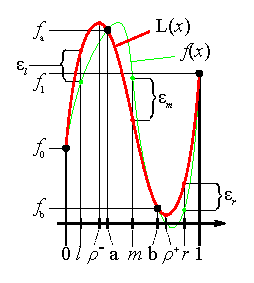
\includegraphics{Images/CubicLagrange.eps}
  \caption[Example Cubic Lagrange Interpolation]
          {Example Cubic Lagrange Interpolation}
  \label{fig:CubicLagrange}
\end{figure}

Figure \ref{fig:CubicLagrange} depicts an example interpolation with many of the elements discussed in this section present.

%% See ./library/InterpolationError.pdf
%% Available from: http://www.math.montana.edu/~davis/Classes/MA442/Sp07/Notes/InterpError.pdf
As may be found in any elementary calculus text the error of an $n^{th}$-order polynomial interpolation of $f(x)$ is given by
\begin{align}
L(x) - f(x) &= -\frac{f^{(n+1)}(c)}{(n+1)!}\prod_{i=0}^n(x - x_i)\\
\label{eq:TaylorError}
            &= \frac{f^{(4)}(c)}{4!}\;x(1-x)(x^2-x+a-a^2)
\end{align}
where $n=3$, $x_i \in \{0,a,1-a,1\}$ and for some $c \in (0,1)$. The largest errors occur at the extrema of the fourth-order polynomial $E(x) = x(1-x)(x^2-x+a-a^2)$ in the error expression. The extrema points are called \emph{ridge-error} points. Solving $E(x)$ for the ridge-error points,
\begin{align*}
\frac{d}{dx}E(x) = 0 \implies 
x = \left\{\frac{1}{2}\left(1\pm\sqrt{2a^2-2a+1}\right), \frac{1}{2}\right\}
\end{align*}
Evaluating $E(x)$ at each ridge-error point yields the unique extrema,
\begin{align*}
\left\{\frac{1}{4}a^2(1-a)^2, -\left(\frac{1-2a}{4}\right)^2\right\}
\end{align*}
Equating the absolute value of the two ridge-point extrema yields the following candidates for $a$,
\begin{align*}
2a(1-a) \equiv 1-2a \implies a = 1 \pm \frac{1}{\sqrt{2}}
\end{align*}
Since $a$ is required to lie in the interval $(0,\frac{1}{2})$ so that $0 < a < b < 1$, the ridge-point values are equated in absolute value by the choice
\begin{align}
a = 1-\frac{1}{\sqrt{2}} \approx 0.29289322
\label{eq:LagrangeInterpolationPoint}
\end{align}
Given this choice of $a$ the ridge-error points are,
\begin{align*}
l &= \frac{1}{2}\left(1-\sqrt{2a^2-2a+1}\right) = \frac{1}{2}\left(1 - \sqrt{2-\sqrt{2}}\right) \approx 0.117317\\
m &= \frac{1}{2}\\
r &= \frac{1}{2}\left(1+\sqrt{2a^2-2a+1}\right) = \frac{1}{2}\left(1 + \sqrt{2-\sqrt{2}}\right) \approx 0.882683
\end{align*}
and the $L(x)$ coefficients are found to be,
\begin{align}
\begin{pmatrix}\alpha_0\\\alpha_1\\\alpha_2\\\alpha_3\end{pmatrix} =
\begin{pmatrix}1&0&0&0\\
-(3+2\sqrt{2})&4+3\sqrt{2}&-(2+\sqrt{2})&1\\
4+4\sqrt{2}&-(10+7\sqrt{2})&8+5\sqrt{2}&-(2+2\sqrt{2})\\
-(2+2\sqrt{2})&6+4\sqrt{2}&-(6+4\sqrt{2})&2+2\sqrt{2}
\end{pmatrix}
\begin{pmatrix}f_0\\f_a\\f_b\\f_1\end{pmatrix}
\label{eq:LagrangeCoefficients}
\end{align}
%% Check the matrix in Python
\begin{comment}
def f(x): return (x-.1)*(x+1)*(x-2)    ## x^3 - 1.1x^2 -1.9x + 0.2

sqrt2 = 1.4142135623730950488016887242096980785696718753769480
a = 0.2928932188134524755991556378951509607151640623115259  ## 1-1/sqrt(2)
b = 1-a;
f0 = f(0); fa = f(a); fb = f(b); f1 = f(1)
a0 =                f0
a1 = -(3+2*sqrt2) * f0 + (4 +3*sqrt2) * fa - (2+  sqrt2) * fb +               f1
a2 =  (4+4*sqrt2) * f0 - (10+7*sqrt2) * fa + (8+5*sqrt2) * fb - (2+2*sqrt2) * f1
a3 = -(2+2*sqrt2) * f0 + (6 +4*sqrt2) * fa - (6+4*sqrt2) * fb + (2+2*sqrt2) * f1
\end{comment}
Let $A_{opt}$ be the matrix in the above equation. Noticing that
\begin{align*}
L(x) = (1,x,x^2,x^3)\;\begin{pmatrix}\alpha_0\\\alpha_1\\\alpha_2\\\alpha_3\end{pmatrix} = (1,x,x^2,x^3)\;A_{opt}\;\mathbf{f}
\end{align*}
it is possible to precompute \emph{ridge-error vectors}, $v_l, v_m, v_r$ corresponding to the ridge-error values $l, m, r$ found above for the sake of computational efficiency. Let
\begin{align*}
\mathbf{v}_k = (1,x_k,x_k^2,x_k^3)\;A_{opt} && \text{ for } && k \in \{l, m, r\}
\end{align*}
The ridge-error vectors are then,
\begin{align}
\mathbf{v}_l &= \frac{1}{4}\left(1+\sqrt{2-\sqrt{2}}, 1+\sqrt{2+\sqrt{2}}, 1-\sqrt{2+\sqrt{2}}, 1-\sqrt{2-\sqrt{2}}\right)^T\\
\mathbf{v}_m &= \frac{1}{4}\left(1-\sqrt{2}, 1+\sqrt{2}, 1+\sqrt{2}, 1-\sqrt{2}\right)^T\\
\mathbf{v}_r &= \frac{1}{4}\left(1-\sqrt{2-\sqrt{2}}, 1-\sqrt{2+\sqrt{2}},1+\sqrt{2+\sqrt{2}}, 1+\sqrt{2-\sqrt{2}}\right)^T
\label{eq:RidgeErrorVectors}
\end{align}
%% For Wolfram|Alpha
\begin{comment}
evaluate 1-x*(3+2*sqrt(2))+x^2*(4+4*sqrt(2)) -x^3*(2+2*sqrt(2)) where x = 1/2*(1-sqrt(2-sqrt(2)))
evaluate 0+x*(4+3*sqrt(2))-x^2*(10+7*sqrt(2))+x^3*(6+4*sqrt(2)) where x = 1/2*(1-sqrt(2-sqrt(2)))
evaluate 0-x*(2+sqrt(2))  +x^2*(8+5*sqrt(2)) -x^3*(6+4*sqrt(2)) where x = 1/2*(1-sqrt(2-sqrt(2)))
evaluate 0+x              -x^2*(2+2*sqrt(2)) +x^3(2+2*sqrt(2))  where x = 1/2*(1-sqrt(2-sqrt(2)))

simplify evaluate 1-x*(3+2*sqrt(2))+x^2*(4+4*sqrt(2)) -x^3*(2+2*sqrt(2)) where x = 1/2
simplify evaluate 0+x*(4+3*sqrt(2))-x^2*(10+7*sqrt(2))+x^3*(6+4*sqrt(2)) where x = 1/2
simplify evaluate 0-x*(2+sqrt(2))  +x^2*(8+5*sqrt(2)) -x^3*(6+4*sqrt(2)) where x = 1/2
simplify evaluate 0+x              -x^2*(2+2*sqrt(2)) +x^3(2+2*sqrt(2))  where x = 1/2

evaluate 1-x*(3+2*sqrt(2))+x^2*(4+4*sqrt(2)) -x^3*(2+2*sqrt(2)) where x = 1/2*(1+sqrt(2-sqrt(2)))
evaluate 0+x*(4+3*sqrt(2))-x^2*(10+7*sqrt(2))+x^3*(6+4*sqrt(2)) where x = 1/2*(1+sqrt(2-sqrt(2)))
evaluate 0-x*(2+sqrt(2))  +x^2*(8+5*sqrt(2)) -x^3*(6+4*sqrt(2)) where x = 1/2*(1+sqrt(2-sqrt(2)))
evaluate 0+x              -x^2*(2+2*sqrt(2)) +x^3(2+2*sqrt(2))  where x = 1/2*(1+sqrt(2-sqrt(2)))
\end{comment}
The ridge-error points and vectors are then used to compute the following set of interpolation errors,
\begin{align}
\epsilon_l &= |f(l) - \mathbf{v}_l^T \mathbf{f}\,|\\
\epsilon_m &= |f(m) - \mathbf{v}_m^T \mathbf{f}\,|\\
\epsilon_r &= |f(r) - \mathbf{v}_r^T \mathbf{f}\,|
\label{eq:RidgeErrorValues}
\end{align}
The \emph{EveryRoot} method uses the above interpolation errors to determine if $L(x)$ is a reliable facsimile to $f(x)$ over the normalized interval $[0,1]$. If $L(x)$ is deemed reliable the \emph{EveryRoot} method requires the extrema points of $L(x)$. These are found by solving the quadratic $L'(x) = 0$ and accepting only real roots, that is,
\begin{align*}
L'(x) &= 3\alpha_3\,x^2 + 2\alpha_2\,x + \alpha_1  = 0\\
\rho &=  -\frac{\alpha_2}{3\alpha_3} \pm \sqrt{\left(\frac{\alpha_2}{3\alpha_3}\right)^2-\frac{\alpha_1}{3\alpha_3}}
\end{align*}
The curvature of $L(x)$ is given by its second derivative,
\begin{align*}
L''(x) = 6\alpha_3\,x + 2\alpha_2
\end{align*}
When $L''(x)$ is evaluated at the extrema, if any, then the \emph{EveryRoot} method can decide if the extrema is near zero and warrents further investigation. Notice, for example, that in figure \ref{fig:CubicLagrange} the objective function $f(x)$ crosses zero even though $L(x)$ does not. The example in the figure has grossly exaggerated error values for $\{\epsilon_l, \epsilon_m, \epsilon_r\}$ and $L(x)$ would certainly be rejected by the \emph{EveryRoot} method as un-reliable. An interesting modification to the \emph{EveryRoot} method presents itself in the case of a reliability rejection; subdivide the interval into three parts, not two, namely $\{(0,a),(a,b),(b,1)\}$. The rationale for this modification is that each of the endpoints has already been evaluated so that $\{f_0, f_a, f_b, f_1\}$ are already in hand.

Notice further from the example depicted in figure \ref{fig:CubicLagrange} that because $L(x)$ is concave at the upper root, $\rho^+$, it seems a good place to initialize a root polishing method. In the figure it appears that a root is already found. This is accidental, but makes the point that even a reliable $L(x)$ should not be taken as a duplicate of the objective $f(x)$.

A rule to consider as a modification to the \emph{EveryRoot} method is if
\begin{align*}
|L(\rho)| < max\{\epsilon_l, \epsilon_m, \epsilon_r\}
\end{align*}
then root polishing should be initiated. A root polisher such as Halley's method, which approximates $f(x)$ with a parabola may best be initiated at the relevant $\rho$ and to bound it by the nearest known neighbors. In the figure the relevant extrema is $\rho^+$ and the bounding interval is $(b,r)$.

\subsubsection{Building the Interpolation Subroutine}

The \emph{EveryRoot} algorithm enters the Lagrange interpolation subroutine when $f_0f_1>0$, that is, the end points are on the same side of zero. The evaluations of $f_0$ and $f_1$ are assumed. The Lagrange interpolation subroutine must evaluate $f(x_a) = f_a$ and $f(x_b) = f_b$ to create the $\mathbf{\alpha}$ polynomial coefficients. Suppose $f_a$ is such that $f_0f_a < 0$, that is, on the other side of zero, then the two subintervals described by the partition $[0,a,1]$, are sent back to the \emph{EveryRoot} method where each is marked as known to contain at least one root.

Continuing with the interpolation subroutine, three more function evaluations at the ridge-error points must be made, namely, $\{f_l, f_m, f_r\}$. The total number of new function evaluations so far is five. If any of the ridge-error evaluations result in a zero crossing the appropriate partition of the investigation interval is sent back to the \emph{EveryRoot} method and each maked as known to contain at least one root. Suppose, for example, only $f_l$ crosses zero such that $f_0f_l < 0$ then the sub-partitition $[0,l,a]$ is sent back with each containing a root and the remaining $[a,1]$ is resent to the interpolation subroutine as an investigation interval since $f_af_1>0$.

At this point it is decided whether the interpolation is reliable. If not, there are five new interval endpoints that cannot be recycled so these become natural investigation subintervals, that is, the initial (normalized) interval is partitioned into six subintervals, $[0,l, a, m, b, r, 1]$ and each is re-fed in turn into the interpolation subroutine.

If the interpolation is deemed reliable then extrema are calculated. Either the extrema are real or not and if real inside the interval or not. If there is no extrema within the interval of positive curvature when $f_0 > 0$ and negative if $f_0 < 0$, in other words, close to zero, then the entire interval $[0,1]$ is marked as containing no roots and the subroutine ends.

If there is an extrema $\rho$ of appropriate curvature then a final function evaluation is made at $f_{\rho} = f(\rho)$. If $f_0f_{\rho}<0$ then the partition $[0,\rho,1]$ is sent back each known to contain a root otherwise the two nearest neighbor points are chosen and the roots of the derivative of the objective $f$ are found. For example in figure \ref{fig:CubicLagrange}, $\rho^+$  is the suggested minima. The nearest neighbors are $\{b, r\}$ and the true minima of $f$ could be left or right of $\rho^+$. 

Suppose the interval $[b,r]$ is suspected of containing the minima. If the endpoints are such that $f'(b) < 0$ and $f'(r)>0$ then a root bounding method applied to $f'$ over $[b,r]$ is used to find $\hat{\rho}$, the true minima of $f$. Otherwise the interpolation subroutine is re-entered over interval $[b,r]$ and the flanking intervals $\{[0,b]$, $[r,1]\}$ are marked as not containing roots. If $\hat{\rho}$ exists and $f_0f(\hat{r})>0$ the interval is declared to no contain a root else the intervals are $\{[b,\hat{\rho}], [\hat{\rho},r]\}$ each sent to the bounded root method since each contains a root. The possibility that $f(\hat{\rho}) \approx 0$ is considered and if true a single root is returned at $\hat{\rho}$.

